\subsection{Güte des Selektivverstärkers}
\begin{table}[h]
	\begin{center}
		\begin{tabular}{ccc}
			Frequenz [kHz] & Ausgansspannung $U_aus$ [mV]\\ \hline
			30	&31\\
			31	&38\\
			32	&52\\
			33	&78\\
			34	&155\\
			34,2&185\\
			34,4&237\\
			34,6&315\\
			34,8&480\\
			35	&755\\
			35,2&685\\
			35,4&430\\
			35,6&300\\
			35,8&220\\
			36	&180\\
			37	&88\\
			38	&58,5\\
			39	&44\\
			40	&35,5\\
		\end{tabular}
		\caption{Güte des Selektivfilters}
		\label{taba}
	\end{center}
\end{table}
\begin{figure}[h]
		\begin{center}
		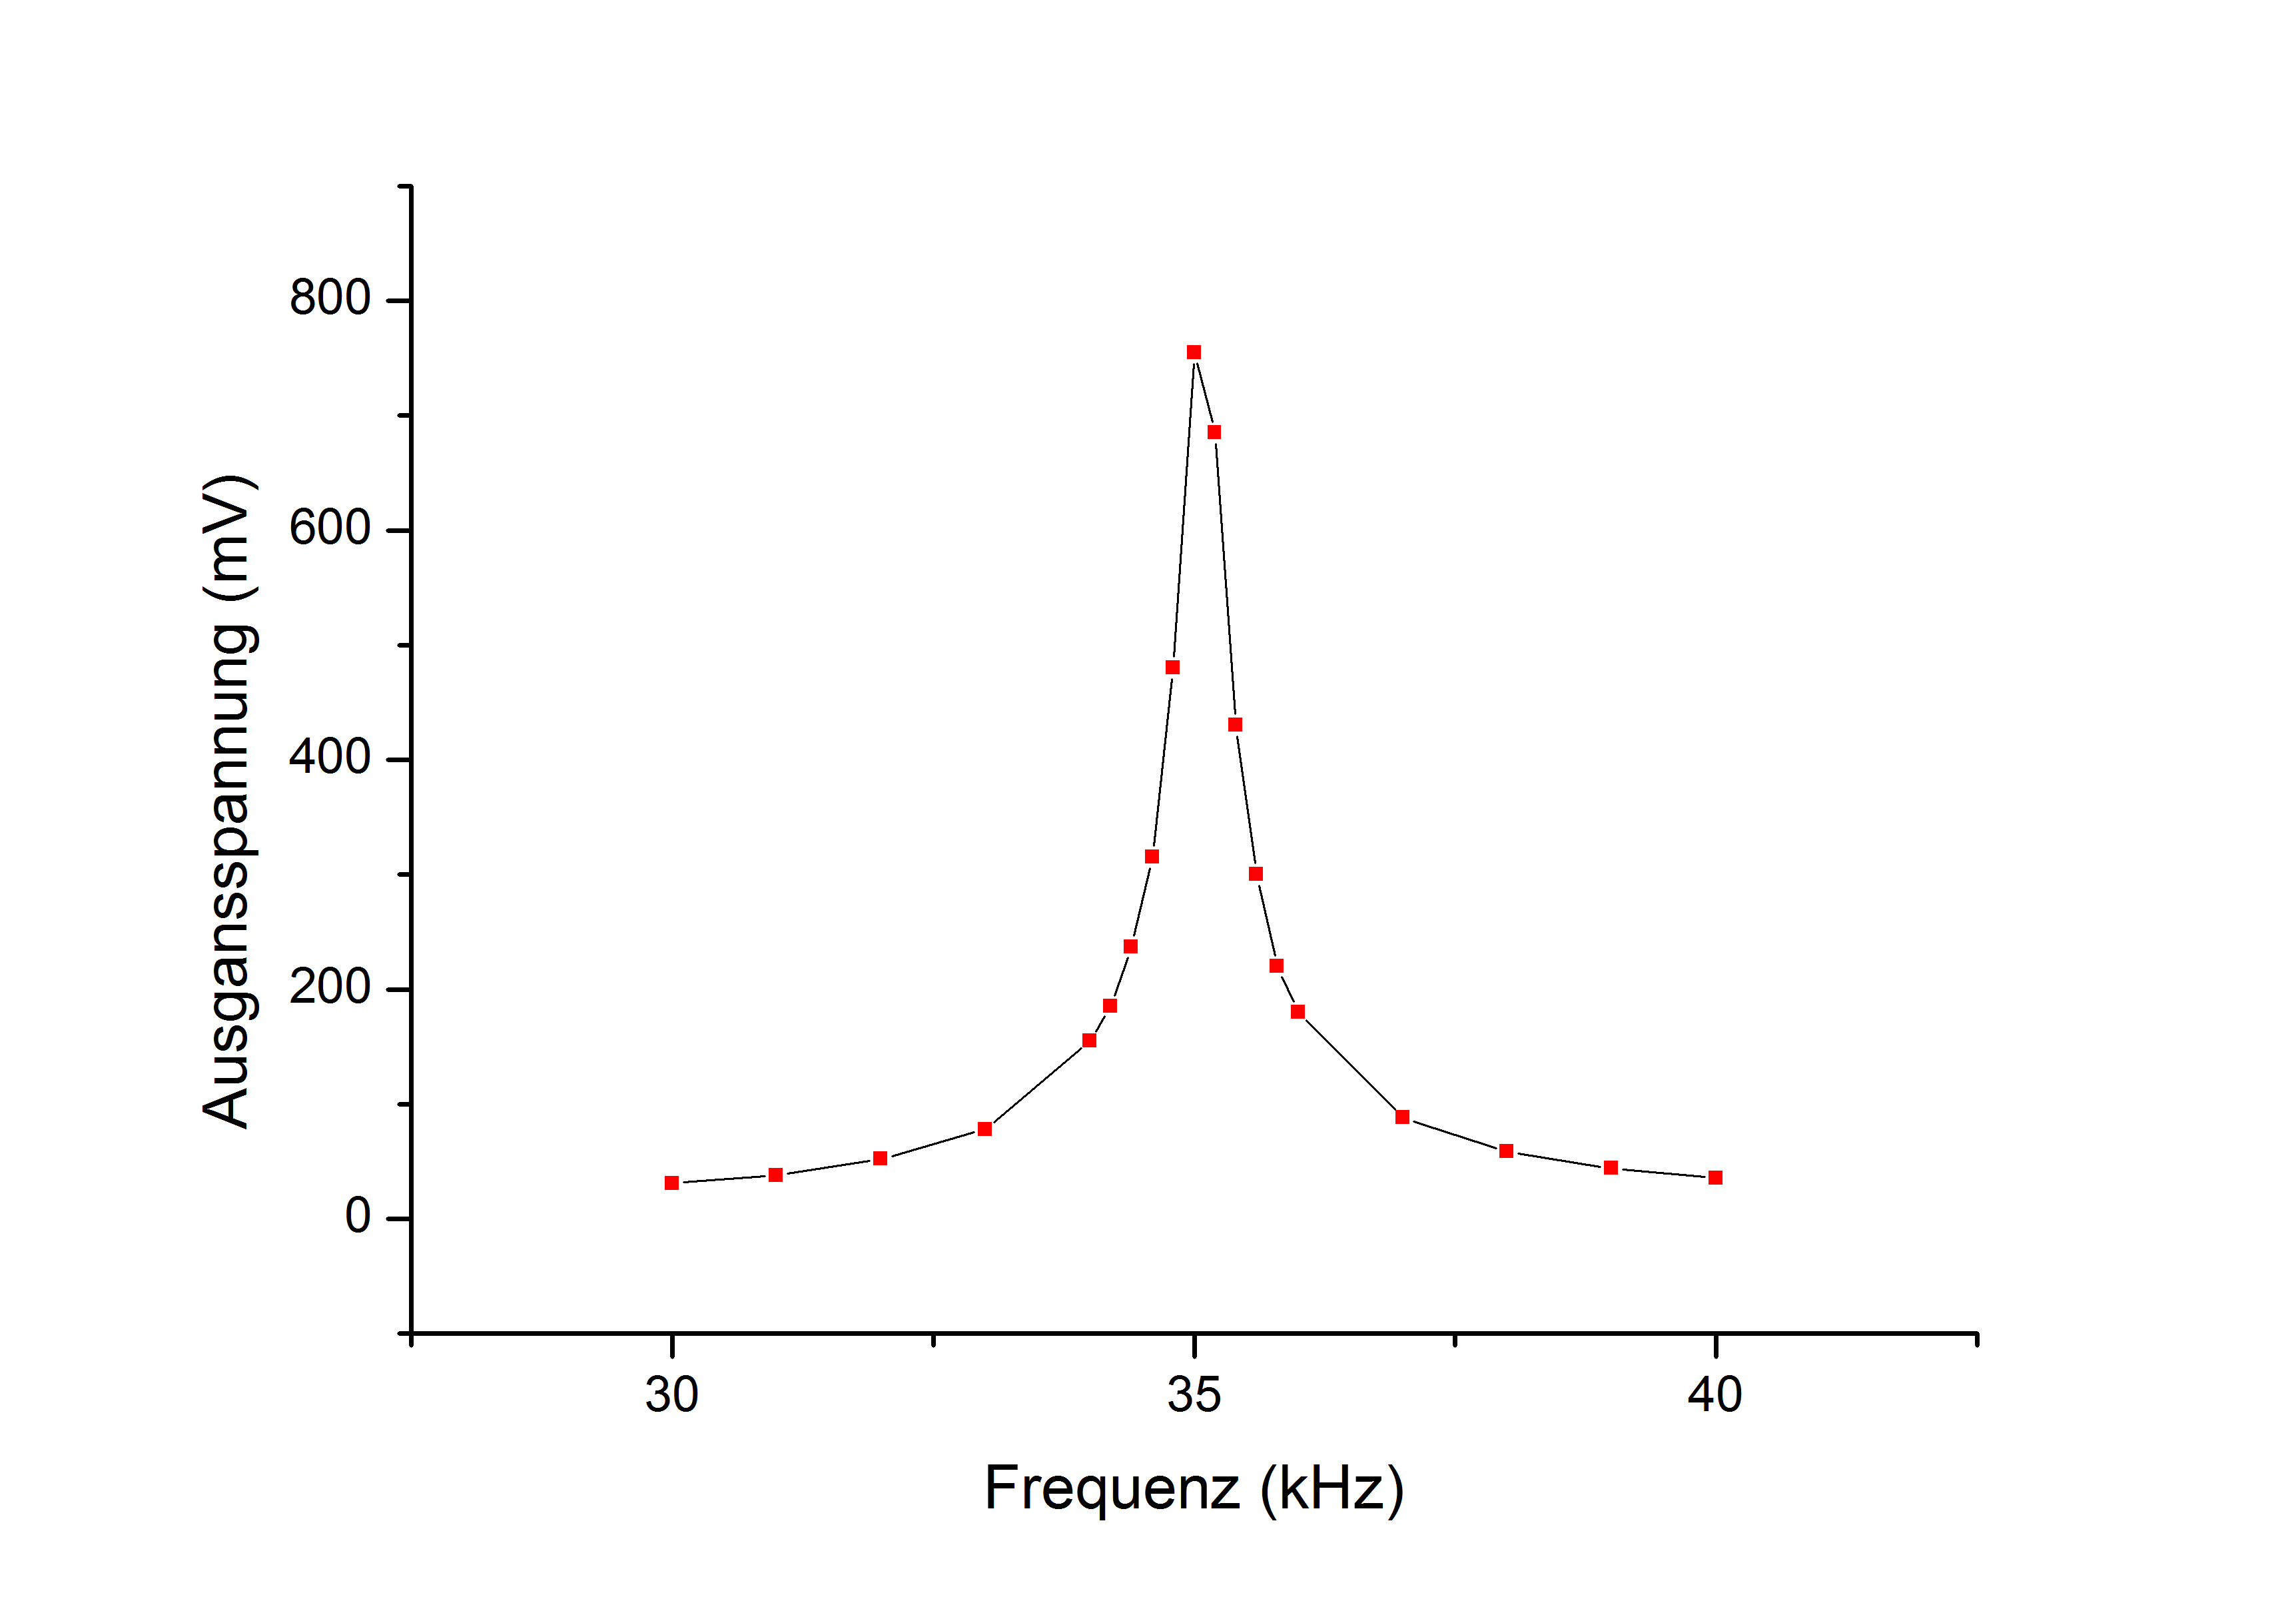
\includegraphics[scale=0.4]{gute.jpg}
		\caption{Güte des Selektivverstärkers}
		\label{gute}
		\end{center}	
\end{figure}

Aus dem Graph \ref{gute} lassen sich die Werte $\nu_-=34,8$,$\nu_0=35,0$ und $\nu_+=35,3$ ablesen. Aus \eqref{eqn:engute} ergibt sich eine Güte von q=70.

\subsection{Probe 1}
Bei der ersten Probe Handelt es sich um $Nd_2O_3$ mit folgenden Werten\cite{tafel}:
\begin{align*}
&J=\frac92&
&g_J=\frac{8}{11}&
&\rho=7,24\frac{g}{cm^3}&
&N=2,59*10^{28}m^{-3}&\\
&M=336,48\frac{\text{g}}{\text{mol}}&
&F=86,6\text{ mm$^2$}&
&Q_{real}=3,00*10^{-4}\text{ m}^2&
\end{align*}
\\
Daraus ergibt sich aus dem Curie'schen Gesetz \eqref{eqn:curie}
$\chi=3,020*10^{-3}$.
\begin{table}[h]
	\begin{center}
		\begin{tabular}{cc|ccc}
			Brückenspannung $U_B$ [mV]&$\chi_{U}*10^-3$ & $\Delta R$ [m$\Omega$]&$R_3[\text{m}\Omega]$&$\chi_R*10^{-3}$\\ \hline
			3,5	&4,493&140&2555&3,165\\
			2,8	&3,594&90&2552&2,037\\
			3	&3,851&100&2550&2,265\\
			3,7	&4,750&155&2600&3,444
		\end{tabular}
		\caption{$Nd_2O_3$}
		\label{tab2}
	\end{center}
\end{table}
Aus der Tabelle \ref{tab2} ergeben sich die gemittelten Werte nach Gleichung \ref{eqmittel},\ref{eqmittelerr}
\begin{align*}
&R_3=2564,25m\Omega&
&U_{Br}=3,25mV&
&\Delta R=(121,25\pm15,60)\text{ m}\Omega&
\end{align*}
Nach \eqref{eqchiu} lässt sich über die Brückenspannung
$\chi_U$
berechnen. \\Gemittelt ergibt sich $\overline\chi_U=4,172*10^{-3}$.
\\
Aus der Widerstandsmessung ergibt sich nach \eqref{eqchir} der gemittelte Wert
$\overline\chi_R=2,728*10^{-3}$.
\begin{align}
\overline x &=\frac{1}{N} \sum_{i=1}^N x_i\label{eqmittel}\\
\Delta \overline x&= (\frac{1}{N^2-N} \sum_{i=1}^N (x_i - \overline x)^2)^{1/2}\label{eqmittelerr}
\end{align}

\subsection{Probe 2}
Bei der zweiten Probe Handelt es sich um $Gd_2O_3$ mit folgenden Werten\cite{tafel}:
\begin{align*}
&J=\frac72&
&g_J=2&
&\rho=7,40\frac{g}{cm^3}&
&N=2,46*10^{28}m^{-3}&\\
&M=362,5\frac{\text{g}}{\text{mol}}&
&F=86,6\text{ mm$^2$}&
&Q_{real}=3,16*10^{-4}\text{ m}^2&
\end{align*}
Daraus ergibt sich nach \eqref{eqn:curie}
$\chi=13,79*10^{-3}$
\begin{table}[h]
	\begin{center}
		\begin{tabular}{c|ccc}
				a	&Radius						&Höhe	&Masse \\ \hline
			Arm		&$(6,850\pm1,765)*10^{-3}$	&0,142	&0,01447$\pm$53,96%\\
			Kopf	&$(1,23\pm0,324)*10^{-2}$	&0,053	&0,01744$\pm$55,11%\\
			Torso	&$(1,82\pm0,25)*10^{-2}$	&0,0975	&0,06991$\pm$31,85%\\
			Bein	&$(8,375\pm1,395)*10^{-3}$	&0,149	&0,02270$\pm$37,00%
		\end{tabular}
		\caption{Messdaten der Trägheitspuppe}
		\label{tab:puppe}
	\end{center}
\end{table}
Aus der Tabelle \ref{tab3} ergeben sich die gemittelten Werte
\begin{align*}
&R_3=2553,75m\Omega&
&U_{Br}=17,25mV&
&\Delta R=(770\pm17,91)\text{m}\Omega&
\end{align*}
Nach \eqref{eqchiu} lässt sich über die Brückenspannung
$\chi_U$
berechnen.\\ Gemittelt ergibt sich $\overline\chi_U=21,01*10^{-3}$.
\\
Aus der Widerstandsmessung ergibt sich nach \eqref{eqchir} der gemittelte Wert
$\overline\chi_R=16,52*10^{-3}$.



\subsection{Probe 3}
Bei der dritten Probe Handelt es sich um $Dy_2O_3$ mit folgenden Werten\cite{tafel}:
\begin{align*}
&J=\frac{15}{2}&
&g_J=\frac43&
&\rho=7,80\frac{g}{cm^3}&
&N=2,52*10^{28}m^{-3}&\\
&M=372,998\frac{\text{g}}{\text{mol}}&
&F=86,6\text{ mm$^2$}&
&Q_{real}=3,09*10^{-4}\text{ m}^2&
\end{align*}
Daraus ergibt sich nach \eqref{eqn:curie} 
$\chi=25,41*10^{-3}$
\begin{table}[h]
	\begin{center}
		\begin{tabular}{cc|ccc}
			Brückenspannung $U_B$ [mV]&$\chi_{U}*10^-3$ & $\Delta R$ [m$\Omega$]&$R_3[\text{m}\Omega]$&$\chi_R*10^{-3}$\\ \hline
			35	&43,66&1655&2555&36,36\\
			36	&44,91&1620&2555&35,60\\
			36,5&45,54&1650&2555&36,25\\
			37	&46,16&1660&2550&36,55
		\end{tabular}
		\caption{$Dy_2O_3$}
		\label{tab4}
	\end{center}
\end{table}
Aus der Tabelle \ref{tab4} ergeben sich die gemittelten Werte
\begin{align*}
&R_3=2553,75m\Omega&
&U_{Br}=36,125mV&
&\Delta R=(1646,25\pm8,98)\text{m}\Omega&
\end{align*}
Nach \eqref{eqchiu} lässt sich über die Brückenspannung
$\chi_U$
berechnen. \\Gemittelt ergibt sich $\overline\chi_U=45,07*10^{-3}$.
\\
Aus der Widerstandsmessung ergibt sich nach \eqref{eqchir} der gemittelte Wert
$\overline\chi_R=36,19*10^{-3}$.\\
Desweiteren war $U_{Sp}=0,9\text{ V}$.
